\documentclass[a4paper,12pt]{article}
\usepackage[utf8]{inputenc}
\usepackage[spanish]{babel}
\usepackage{color}
\usepackage{parskip}
\usepackage{graphicx}
\usepackage{multirow}
\usepackage{listings}
\usepackage{vmargin}
\graphicspath{ {imagenes/} }
\definecolor{mygreen}{rgb}{0,0.6,0}
\definecolor{lbcolor}{rgb}{0.9,0.9,0.9}
\usepackage{epstopdf}

\lstset{
backgroundcolor=\color{lbcolor},
    tabsize=4,    
%   rulecolor=,
    language=[ANSI]C,
        basicstyle=\tiny,
        aboveskip={1.5\baselineskip},
        columns=fixed,
        showstringspaces=false,
        extendedchars=false,
        breaklines=true,
        prebreak = \raisebox{0ex}[0ex][0ex]{\ensuremath{\hookleftarrow}},
        frame=single,
        showtabs=false,
        showspaces=false,
        showstringspaces=false,
        identifierstyle=\ttfamily,
        keywordstyle=\color[rgb]{0,0,1},
        commentstyle=\color[rgb]{0.026,0.112,0.095},
        stringstyle=\color{red},
        numberstyle=\color[rgb]{0.205, 0.142, 0.73},
%        \lstdefinestyle{C++}{language=C++,style=numbers}’.
}

\begin{document}
\title{Cuestionario Capítulos 3 y 4}
\author{
Christofer Fabián Chávez Carazas \\
\small{Universidad Nacional de San Agustín} \\
\small{Algoritmos Paralelos}
}

\maketitle

\section{Capítulo 3}

\begin{enumerate}
\item \textbf{What happens in the greetings program if, instead of strlen(greeting) + 1,
we use strlen(greeting) for the length of the message being sent by processes 1, 2, ... , comm\_sz−1?
What happens if we use MAX\_STRING instead of strlen(greeting)+1? Can you explain these results?}

Toda cadena de caracteres termina con un null ('\textbackslash 0'). La función \textit{strlen()} cuenta los caracteres hasta llegar
al null y retorna el tamaño de la cadena sin contar el null. Se coloca el +1 para que al momento de enviar el mensaje se copie
toda la cadena más el null. La función \textit{printf()} imprime el los caracteres hasta encontrar un null. Si nosotros
no colocamos el +1, el null no se va a copiar, y al momento de imprimir la cadena, ésta se imprimiría con basura al final.
Si nosotros usamos MAX\_STRING, sí estaríamos copiando el null, pero también basura; no se imprimiría dicha basura, pero se
estaría perdiendo tiempo copiándola.

\item \textbf{Modify the trapezoidal rule so that it will correctly estimate the integral 
even if comm\_sz doesn’t evenly divide n. (You can still assume that n ≥ comm\_sz.)}

Al código original agregarle lo siguiente:

\begin{lstlisting}
if(my_rank == comm_sz -1) local_n = n / comm_sz + (n % comm_sz);
else local_n = n / comm_sz;
local_a = a + my_rank * (n/comm_sz) * h;
local_b = local_a + local_n * h;
local_int = Trap(local_a, local_b, local_n, h);
\end{lstlisting}

La idea es darle al último proceso lo que sobra de trapecios para poder conseguir el resultado exacto.

\item \textbf{Determine which of the variables in the trapezoidal rule program are local and which are global}

Las variables globales son las siguientes:

\begin{itemize}
 \item El número de divisiones.
 \item El número de prosesos.
 \item El rango de la función (a y b).
 \item El tamaño de cada trapecio.
\end{itemize}

Las variables locales son las siguientes:

\begin{itemize}
 \item El número de trapecios.
 \item El rango que le toca a cada proceso (local\_a y local\_b).
 \item La suma local.
 \item La suma total para el proceso 0.
 \item El id de cada proceso.
\end{itemize}

\item \textbf{Modify the program that just prints a line of output from each process (mpi\_output.c) so that the output 
is printed in process rank order: process 0s output first, then process 1s, and so on.}

El código es el que continua:

\begin{lstlisting}
#include <stdio.h>
#include <mpi.h>

int main(void) {
	int my_rank, comm_sz;
	MPI_Init(NULL, NULL);
	MPI_Comm_size(MPI_COMM_WORLD, &comm_sz);
	MPI_Comm_rank(MPI_COMM_WORLD, &my_rank);
	if(my_rank != 0){
		MPI_Send(&my_rank,1,MPI_INT,0,0,MPI_COMM_WORLD);
	}
	else{
		printf("Proc %d of %d > Does anyone have a toothpick?\n", my_rank, comm_sz);	
		for(int i = 1; i < comm_sz; i++){
			int res;
			MPI_Recv(&res,1,MPI_INT,i,0,MPI_COMM_WORLD,MPI_STATUS_IGNORE);
			printf("Proc %d of %d > Does anyone have a toothpick?\n", i, comm_sz);
		}
	}
	MPI_Finalize();
	return 0;
}
\end{lstlisting}

Para imprimir todo en orden la solución es dejar que sólo el proceso 0 imprima todo. Los demás proceso envian un mensaje
para avisarle al proceso 0 que imprima lo suyo. El proceso 0 mediante un \textit{for} imprime todo en orden. 

\item \textbf{In a binary tree, there is a unique shortest path from each node to the root.Thelength of this path
is often called the depth of the node. A binary tree in which every nonleaf has two children is called a full binary tree,
and a full binary tree in which every leaf has the same depth is sometimes called a complete binary tree. 
Use the principle of mathematical induction to prove that if T is a complete binary tree with n leaves, 
then the depth of the leavesis $log_{2} (n).$}

En los árboles binarios completos, el número de hojas se va multiplicando por dos cada vez que el arbol crece, esto nos
deja con lo siguiente:

$$2^{k} = n$$
$$2^{k+1} = n * 2$$
$$2^{k} * 2 = n * 2$$
$$n * 2 = n * 2$$

\item {\textbf{Suppose comm\_sz = 4 and suppose that x is a vector with n = 14 components.} \\
\begin{enumerate}
 \item \textbf{How would the components of x be distributed among the processes in a
program that used a block distribution?}
\item \textbf{How would the components of x be distributed among the processes in a
program that used a cyclic distribution?}
\item \textbf{How would the components of x be distributed among the processes in a
program that used a block-cyclic distribution with blocksize b = 2?}
\end{enumerate}
\textbf{You should try to make your distributions general so that they could be used regardless of what comm\_sz and n are.
You should also try to make your distributions ``fair'' so that if q and r are any two processes, the difference between
the number of components assigned to q and the number of components assigned to r is as small as possible.}
}

\begin{enumerate}
 \item Por bloque se le daría a los 3 primeros proceso 3 valores del vector, y al proceso 4 se le daría 3 y los 2 que restan.
 \item Ciclicamente se le daría un valor a cada proceso hasta que el vector se termine. El primer proceso tendría 4, el segundo
 tendría 4, el tercero; 3 y el ccuarto; 3.
 \item Cliclicamente por bloque con b = 2 se le daría dos valores a cada proceso haste que el vector se termine. El primer, segundo
  y tercer proceso tendrían 4 valores, mientras que el cuarto sólo tendría 2.
\end{enumerate}

\item \textbf{What do the various MPI collective functions do if the communicator contains a single process?}

Lo ideal sería que el MPI detecte que sólo hay un proceso y que convierta el programa parallelo en uno serial. Pero como eso
no pasa, simplemente copia lo que tiene que copiar. Por ejemplo, si utilizamos \textit{MPI\_Scatter()} con un sólo proceso, todo
el vector origen se copiaría en el vector destino de ese proceso sin dividirlo.

\item {\textbf{Suppose comm\_sz = 8 and n = 16}
 \begin{enumerate}
  \item \textbf{Draw a diagram that shows how MPI\_Scatter can be implemented using tree-structured communication 
  with comm\_sz processes when process 0 needs to distribute an array containing n elements.}
  \item \textbf{ Draw a diagram that shows how MPI\_Gather can be implemented using tree-structured communication 
  when an n-element array that has been distributed among comm\_sz processes needs to be gathered onto process 0.}
 \end{enumerate}
}

\begin{center}
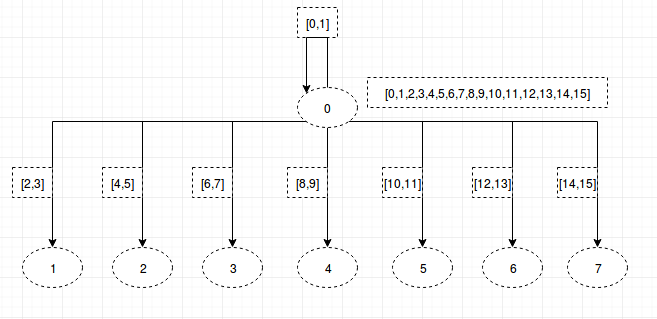
\includegraphics[scale = 0.5]{8_1.png} \par
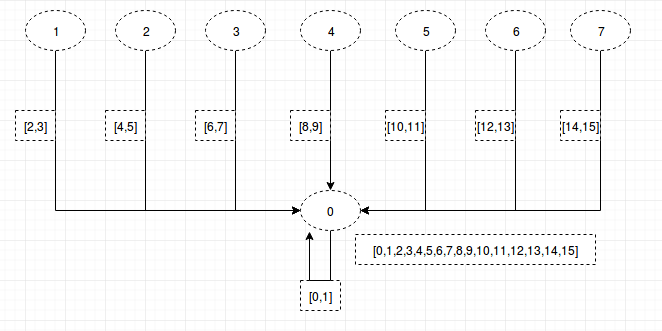
\includegraphics[scale = 0.5]{8_2.png}
\end{center}

\item \textbf{Write an MPI program that implements multiplication of a vector by a scalar and dot product. 
The user should enter two vectors and a scalar, all of which are read in by process 0 and distributed among 
the processes. The results are calculated and collected onto process 0, which prints them. You can assume
that n, the order of the vectors, is evenly divisible by comm\_sz.}

El programa es el siguiente:

\begin{lstlisting}
#include <stdio.h>
#include <stdlib.h>
#include <mpi.h>

#define BUFF_SIZE 10

int multiDot(int * vec1, int * vec2, int size){
	int res = 0;
	for(int i = 0; i < size; i++){
		res += vec1[i] * vec2[i];
	}
	return res;
}

int * multiScalar(int * vec, int scalar, int size){
	int * res = (int*) malloc(sizeof(int) * size);
	for(int i = 0; i < size; i++){
		res[i] = vec[i] * scalar;
	}
	return res;
}

void printVec(int * vec, int size){
	for(int i = 0; i < size; i++){
		printf("%d ", vec[i]);
	}
	printf("\n");
}

int main(){
	int my_rank;
	int comm_sz;
	int n = 4;
	int * vec1 = NULL;
	int * vec2 = NULL;
	int * local_vec1;
	int * local_vec2;
	int * res_scalar1;
	int * res_scalar2;
	int res_dot;
	int scalar;
	int local_n;
	int total_res_dot;
	int * total_res_scalar1;
	int * total_res_scalar2;
	MPI_Init(NULL,NULL);
	MPI_Comm_size(MPI_COMM_WORLD,&comm_sz);
	MPI_Comm_rank(MPI_COMM_WORLD,&my_rank);
	if(my_rank == 0){
		char buff[BUFF_SIZE];
		printf("Tamaño de n->%d\n", n);
		vec1 = (int*) malloc(sizeof(int) * n);
		vec2 = (int*) malloc(sizeof(int) * n);
		int temp = 0;
		printf("Ingrese el vector 1->");
		for(int i = 0; i < n; i++){
			fgets(buff,BUFF_SIZE,stdin);
			temp = atoi(buff);
			vec1[i] = temp;
		}
		printf("Ingrese el vector 2->");
		for(int i = 0; i < n; i++){
			fgets(buff,BUFF_SIZE,stdin);
			temp = atoi(buff);
			vec2[i] = temp;
		}
		printf("Ingrese el scalar->");
		fgets(buff,BUFF_SIZE,stdin);
		scalar = atoi(buff);
	}
	local_n = n / comm_sz;
	local_vec1 = (int*) malloc(sizeof(int) * local_n);
	local_vec2 = (int*) malloc(sizeof(int) * local_n);
	MPI_Scatter(vec1,local_n,MPI_INT,local_vec1,local_n,MPI_INT,0,MPI_COMM_WORLD);
	MPI_Scatter(vec2,local_n,MPI_INT,local_vec2,local_n,MPI_INT,0,MPI_COMM_WORLD);
	if(my_rank == 0) {
		for(int i = 1; i < comm_sz; i++){
			MPI_Send(&scalar,1,MPI_INT,i,0,MPI_COMM_WORLD);
		}
	}
	else MPI_Recv(&scalar,1,MPI_INT,0,0,MPI_COMM_WORLD,MPI_STATUS_IGNORE);
	res_scalar1 = multiScalar(local_vec1,scalar,local_n);
	res_scalar2 = multiScalar(local_vec2,scalar,local_n);
	res_dot = multiDot(local_vec1,local_vec2,local_n);
	MPI_Reduce(&res_dot,&total_res_dot,1,MPI_INT,MPI_SUM,0,MPI_COMM_WORLD);
	total_res_scalar1 = (int*) malloc(sizeof(int) * n);
	total_res_scalar2 = (int*) malloc(sizeof(int) * n);
	MPI_Gather(res_scalar1,local_n,MPI_INT,total_res_scalar1,local_n,MPI_INT,0,MPI_COMM_WORLD);
	MPI_Gather(res_scalar2,local_n,MPI_INT,total_res_scalar2,local_n,MPI_INT,0,MPI_COMM_WORLD);
	if(my_rank == 0){
		printf("Resultado del producto punto->%d\n",total_res_dot);
		printf("Vector1->");
		printVec(total_res_scalar1,n);
		printf("Vector2->");
		printVec(total_res_scalar2,n);
	}
	MPI_Finalize();
	return 0;

}
\end{lstlisting}

\item \textbf{In the Read vector function shown in Program 3.9, we use local\_n as the actual argument for two
of the formal arguments to MPI\_Scatter: send\_count and recv\_count. Why is it OK to alias these arguments?}

Porque el argumento recv\_count lo utilizan todos los procesos al momento de recivir la data, pero el argumento
send\_count sólo lo utiliza el proceso que envía la información.

\item{\textbf{Finding prefix sums is a generalization of global sum. Rather than simply finding the
sum of n values, }
$$x_{0}+x_{1}+...+x_{n-1}$$
\textbf{the prefix sums are the n partial sums}
$$x_{0},x_{0}+x_{1},x_{0}+x_{1}+x_{2},...,x_{0}+x_{1}+...+x_{n-1}$$
\begin{enumerate}
 \item \textbf{Devise a serial algorithm for computing the n prefix sums of an array with n elements.}
 \item \textbf{Parallelize your serial algorithm for a system with n processes, each of which is storing
 one of the x i s.}
 \item \textbf{Suppose $n = 2^{k}$ for some positive integer k. Can you devise a serial algorithm and a 
 parallelization of the serial algorithm so that the parallel algorithm requires only k communication phases?}
 \item \textbf{MPI provides a collective communication function, MPI Scan , that can be used to compute prefix sums:
 It operates on arrays with count elements; both sendbuf\_p and recvbuf\_p should refer to blocks of count
 elements of type datatype . The op argument is the same as op for MPI Reduce . Write an MPI program that
 generates a random array of count elements on each MPI process, finds the prefix sums, and prints the results.}
\end{enumerate}

}

\begin{enumerate}
 \item Primer programa:
\begin{lstlisting}
#include <stdio.h>
#include <stdlib.h>
#include "../utils.h"

int main(){
	int n = 10;
	int * vec = getRandomVector(n);
	int * res = malloc(sizeof(int) * n);
	int sum = 0;
	printVector(vec,n);
	for(int i = 0; i < n; i++){
		sum = 0;
		for(int j = 0; j <= i; j++){
			sum += vec[j];
		}
		res[i] = sum;
	}
	printVector(res,n);
}
\end{lstlisting}
  \item Segundo programa:
\begin{lstlisting}
#include <stdio.h>
#include <stdlib.h>
#include "../utils.h"
#include <mpi.h>

int getPrefixSum(int * vector, int size){
	int res = 0;
	for(int i = 0; i < size; i++){
		res += vector[i];
	}
	return res;
}

int main(){
	int my_rank;
	int comm_sz;
	MPI_Init(NULL,NULL);
	MPI_Comm_size(MPI_COMM_WORLD,&comm_sz);
	MPI_Comm_rank(MPI_COMM_WORLD,&my_rank);
	int my_random = rand() % RAND_RANGE_NUM;
	int res = 0;
	int * vector = (int *) malloc(sizeof(int) * (my_rank + 1));
	int * vector_res = (int *) malloc(sizeof(int) * comm_sz);
	vector[my_rank] = my_random;
	if(my_rank == 0) MPI_Send(&my_random,1,MPI_INT,my_rank + 1,0,MPI_COMM_WORLD);
	else if(my_rank == comm_sz -1) MPI_Recv(vector,my_rank,MPI_INT,my_rank - 1,0,MPI_COMM_WORLD,MPI_STATUS_IGNORE);
	else{
		MPI_Recv(vector,my_rank,MPI_INT,my_rank - 1,0,MPI_COMM_WORLD,MPI_STATUS_IGNORE);
		MPI_Send(vector,my_rank + 1,MPI_INT,my_rank + 1,0,MPI_COMM_WORLD);
	}
	res = getPrefixSum(vector,my_rank + 1);
	MPI_Gather(&res,1,MPI_INT,vector_res,1,MPI_INT,0,MPI_COMM_WORLD);
	if(my_rank == comm_sz - 1) printVector(vector,comm_sz);
	if(my_rank == 0) printVector(vector_res,comm_sz);
	MPI_Finalize();
	return 0;
}
\end{lstlisting}
 \item Si se puede, si es que se reparte el vector en forma de arbol.
 \item Tercer programa:
\begin{lstlisting}
#include <stdio.h>
#include <stdlib.h>
#include "../utils.h"
#include <mpi.h>

int main(){
	int my_rank;
	int comm_sz;
	int n = 10;
	MPI_Init(NULL,NULL);
	MPI_Comm_size(MPI_COMM_WORLD,&comm_sz);
	MPI_Comm_rank(MPI_COMM_WORLD,&my_rank);
	int * vector = getRandomVector(n);
	int * vector_res = (int*) malloc(sizeof(int) * n);
	int res;
	MPI_Scan(vector,vector_res,n,MPI_INT,MPI_SUM,MPI_COMM_WORLD);
	if(my_rank == 0){
		printVector(vector,n);
	}
	if(my_rank == 1) printVector(vector_res,n);
	MPI_Finalize();
	return 0;
}
\end{lstlisting}

\end{enumerate}

\item{\textbf{An alternative to a butterfly-structured allreduce is a ring-pass structure. In a ring-pass, 
if there are p processes, each process q sends data to process q + 1, except that process p − 1 
sends data to process 0. This is repeated until each process has the desired result. Thus, we can
implement allreduce with the following code:}

\begin{lstlisting}
sum = temp val = my val;
for (i = 1; i < p; i++) {
  MPI Sendrecv replace(&temp val, 1, MPI INT, dest,
  sendtag, source, recvtag, comm, &status);
  sum += temp val;
}
\end{lstlisting}

\begin{enumerate}
 \item \textbf{Write an MPI program that implements this algorithm for allreduce. How does its performance
 compare to the butterfly-structured allreduce?}
 \item \textbf{Modify the MPI program you wrote in the first part so that it implements prefix sums.}
\end{enumerate}
}

\begin{enumerate}
 \item Primer programa:
\begin{lstlisting}
#include <stdlib.h>
#include <stdio.h>
#include "time.h"
#include <mpi.h>

int main(){
	int my_rank;
	int comm_sz;
	MPI_Init(NULL,NULL);
	MPI_Comm_size(MPI_COMM_WORLD,&comm_sz);
	MPI_Comm_rank(MPI_COMM_WORLD,&my_rank);
	int my_val = my_rank + 1;
	int sum = 0;
	int temp_val = 0;
	temp_val = my_val;
	sum = temp_val;
	int des = (my_rank + 1) % comm_sz;
	int source = my_rank - 1;
	if(source == -1) source = comm_sz -1;
	for(int i = 1; i < comm_sz; i++){
		MPI_Sendrecv_replace(&temp_val,1,MPI_INT,des,i,source,i,MPI_COMM_WORLD,MPI_STATUS_IGNORE);
		sum += temp_val;
	}
	printf("%d->%d\n",sum,my_rank);
	MPI_Finalize();
	return 0;
}
\end{lstlisting}
\item Segundo Programa:
\begin{lstlisting}

\end{lstlisting}
\end{enumerate}

\item \textbf{MPI Scatter and MPI Gather have the limitation that each process must send or receive the
same number of data items. When this is not the case, we must use the MPI functions MPI\_Gatherv and
MPI\_Scatterv . Look at the man pages for these functions, and modify your vector sum, dot product program
so that it can correctly handle the case when n isn’t evenly divisible by comm\_sz.}

El código se muestra a continuación:

\begin{lstlisting}
#include <stdio.h>
#include <stdlib.h>
#include <mpi.h>
#include "../utils.h"

int suma(int * vector, int size){
	int res = 0;
	for(int i = 0; i < size; i++){
		res += vector[i];
	}
	return res;
}

int main(){
	int my_rank;
	int comm_sz;
	int n = 10;
	MPI_Init(NULL,NULL);
	MPI_Comm_size(MPI_COMM_WORLD,&comm_sz);
	MPI_Comm_rank(MPI_COMM_WORLD,&my_rank);
	int * vector = getRandomVector(n);
	int * dis = (int*) malloc(sizeof(int) * comm_sz);
	int * scounts = (int*) malloc(sizeof(int) * comm_sz);
	int local_n = 0;
	int total_res;
	if(my_rank != comm_sz - 1) local_n = n / comm_sz;
	else local_n = (n / comm_sz) + (n % comm_sz);
	int * local_vector = (int *) malloc(sizeof(int) * local_n);
	for(int i = 0; i < comm_sz; i++){
		dis[i] = i * local_n;
		if(i != comm_sz - 1) scounts[i] = local_n;
		else scounts[i] = local_n + (n % comm_sz);
	}
	MPI_Scatterv(vector,scounts,dis,MPI_INT,local_vector,local_n,MPI_INT,0,MPI_COMM_WORLD);
	int res = suma(local_vector,local_n);
	MPI_Reduce(&res,&total_res,1,MPI_INT,MPI_SUM,0,MPI_COMM_WORLD);
	if(my_rank == 0) {
		printVector(vector,n);
		printf("%d\n",total_res);
	}


	MPI_Finalize();
	return 0;
}
\end{lstlisting}

\item {
  \begin{enumerate}
   \item \textbf{Write a serial C program that defines a two-dimensional array in the main function.
   Just use numeric constants for the dimensions: int two\_d[3][4]; Initialize the array in
   the main function. After the array is initialized, call a function that attempts to print the array.
   The prototype for the function should look something like this. 
   void Print\_two\_d(int two\_d[][], int rows, int cols); After writing the function try
   to compile the program. Can you explain why it won’t compile?}
   \item \textbf{After consulting a C reference (e.g., Kernighan and Ritchie [29]), modify the program
   so that it will compile and run, but so that it still uses a two- dimensional C array.}
   
  \end{enumerate}
}

\begin{enumerate}
 \item Bota un error de compilación diciendo que el tipo de la matriz está incompleto. Porque el tamaño de una fila
 de la matriz es desconocido. Se tiene que especificar los tamaños de todas la dimensiones, excepto 
 la más a la izquierda utilizando expresiones constantes.
 \item A continuación se muestra el código arreglado:
\begin{lstlisting}
#include <stdio.h>
#include <stdlib.h>

void print_two_d(int  two_d[][4], int rows, int cols){
	for(int i = 0; i < rows; i++){
		for(int j = 0; j < cols; j++){
			printf("%d ", two_d[i][j]);
		}
		printf("\n");
	}
	printf("\n");
}


int main(){
	int two_d[3][4];
	for(int i = 0; i < 3; i++){
		for(int j = 0; j < 4; j++){
			two_d[i][j] = j;
		}
	}
	print_two_d(two_d, 3 , 4);
}  
\end{lstlisting}
\end{enumerate}

\item \textbf{What is the relationship between the “row-major” storage for two-dimensional arrays that
we discussed in Section 2.2.3 and the one-dimensional storage we use in Section 3.4.9?}

Cuando la matriz es representada normalmente, cuando se trae un valor de la cache se trae toda la fila almacenada.
En cambio cuando la matriz es representado en forma de vector, cuando se trae un valor de la cache, se traería todo
el vector, o al menos lo que quepa del vector en la cache.

\item \textbf{Suppose comm\_sz = 8 and the vector $x = (0, 1, 2, . . . , 15)$ has been distributed
among the processes using a block distribution. Draw a diagram illustrating the steps in a butterfly
implementation of allgather }

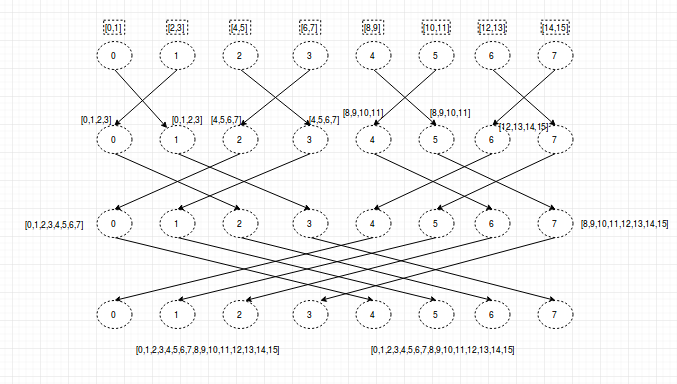
\includegraphics[scale = 0.6]{16.png}

\item{ \textbf{MPI\_Type\_contiguous can be used to build a derived datatype from a collection of contiguous
elements in an array. Its syntax is}

\begin{lstlisting}
int MPI_Type_contiguous(
  int count /∗ in ∗/,
  MPI_Datatype old_mpi t /∗ in ∗/,
  MPI_Datatype∗ new_mpi t p /∗ out ∗);
\end{lstlisting}

\textbf{Modify the Read\_vector and Print\_vector functions so that they use an MPI datatype created by
a call to MPI\_Type\_contiguous and a count argument of 1 in the calls to MPI\_Scatter and MPI\_Gather.}

}

El código es el siguiente:

\begin{lstlisting}
#include <stdio.h>
#include <stdlib.h>
#include <mpi.h>
#include "../utils.h"

int main(){
	int my_rank;
	int comm_sz;
	int n = 10;
	MPI_Init(NULL,NULL);
	MPI_Comm_size(MPI_COMM_WORLD,&comm_sz);
	MPI_Comm_rank(MPI_COMM_WORLD,&my_rank);
	MPI_Datatype data;
	int local_n = n / comm_sz;
	int * vector = getRandomVector(n);
	int * local_vector = malloc(sizeof(int) * local_n);
	int * res = malloc(sizeof(int) * n);
	MPI_Type_contiguous(local_n,MPI_INT,&data);
	MPI_Type_commit(&data);
	MPI_Scatter(vector,1,data,local_vector,1,data,0,MPI_COMM_WORLD);

	for(int i = 0; i < local_n; i++){
		local_vector[i] = local_vector[i] * 2;
	}
	MPI_Gather(local_vector,1,data,res,1,data,0,MPI_COMM_WORLD);

	if(my_rank == 0){
		printVector(vector,n);
		printVector(res,n);
	}


	MPI_Finalize();
	return 0;
}
\end{lstlisting}

\item{\textbf{MPI\_Type\_vector can be used to build a derived datatype from a collection of blocks of
elements in an array as long as the blocks all have the same size and they’re equally spaced. Its syntax is:}

\begin{lstlisting}
int MPI Type vector(
  int count /∗ in ∗/,
  int blocklength /∗ in ∗/,
  int stride /∗ in ∗/,
  MPI_Datatype old_mpi_t /∗ in ∗/,
  MPI_Datatype∗ new_mpi_t_p /∗ out ∗/);
\end{lstlisting}

\textbf{For example, if we had an array x of 18 doubles and we wanted to build a type corresponding to
the elements in positions 0, 1, 6, 7, 12, 13, we could call: int MPI\_Type\_vector(3, 2, 6,
MPI\_DOUBLE, \&vect\_mpi\_t); since the type consists of 3 blocks, each of which has 2 elements, and the
spacing between the starts of the blocks is 6 doubles. Write Read\_vector and Print\_vector functions
that will allow process 0 to read and print, respectively, a vector with a block-cyclic distribution. But
beware! Do not use MPI\_Scatter or MPI\_Gather. There is a technical issue involved in using these
functions with types created with MPI\_Type\_vector. (See, for example, [23].) Just use a loop of
sends on process 0 in Read vector and a loop of receives on process 0 in Print\_vector. The other processes
should be able to complete their calls to Read\_vector and Print\_vector with a single call to
MPI\_Recv and MPI\_Send. The communication on process 0 should use a derived datatype created
by MPI\_Type\_vector. The calls on the other processes should just use the count argument to the
communication function, since they’re receiving/sending elements that they will store in 
contiguous array locations.}
}

El código es el siguiente:

\begin{lstlisting}
#include <stdio.h>
#include <stdlib.h>
#include <mpi.h>
#include "../utils.h"

int main(){
	int my_rank;
	int comm_sz;
	int n = 10;
	MPI_Init(NULL,NULL);
	MPI_Comm_size(MPI_COMM_WORLD,&comm_sz);
	MPI_Comm_rank(MPI_COMM_WORLD,&my_rank);
	MPI_Datatype data;
	int local_n  = n / comm_sz;
	int * vector = getRandomVector(n);
	int * local_vector = (int*) malloc(sizeof(int) * local_n);
	int * res_vector = (int*) malloc(sizeof(int) * n);
	MPI_Type_vector(1,local_n,n + 1,MPI_INT,&data);
	MPI_Type_commit(&data);
	if(my_rank == 0){
		printVector(vector,n);
		for(int i = 0; i < local_n;i++){
			local_vector[i] = vector[i];
		}
		for(int i = 1; i < comm_sz; i++){
			MPI_Send(&vector[i * local_n],1,data,i,0,MPI_COMM_WORLD);
		}
	}
	else{
		MPI_Recv(local_vector,1,data,0,0,MPI_COMM_WORLD,MPI_STATUS_IGNORE);
	}

	for(int i = 0; i < local_n; i++){
		local_vector[i] = local_vector[i] * 2;
	}

	if(my_rank != 0){
		MPI_Send(local_vector,1,data,0,0,MPI_COMM_WORLD);
	}
	else{
		for(int i = 0; i < local_n; i++){
			res_vector[i] = local_vector[i];
		}
		for(int i = 1; i < comm_sz; i++){
			MPI_Recv(&res_vector[i * local_n],1,data,i,0,MPI_COMM_WORLD,MPI_STATUS_IGNORE);
		}
		printVector(res_vector,n);
	}
	MPI_Finalize();
	return 0;
}
\end{lstlisting}

\item{\textbf{MPI\_Type\_indexed can be used to build a derived datatype from arbitrary array elements. Its syntax is:}
\begin{lstlisting}
int MPI Type indexed(
  int count		       /*in*/
  int array_of_blocklengths[]  /*in*/,
  int array_of_displacements[] /*in*/,
  MPI_Datatype old_mpi_t       /*in*/,
  MPI_Datatype∗ new_mpi_t_p)   */out*/);
\end{lstlisting}
\textbf{Unlike MPI\_Type\_create struct , the displacements are measured in units of old\_mpi\_t not bytes.
Use MPI\_Type\_indexed to create a derived datatype that corresponds to the upper triangular part of a square matrix.
For example, in the 4 x 4 matrix the upper triangular part is the elements 0, 1, 2, 3, 5, 6, 7, 10, 11, 15. Process 
0 should read in an n x n matrix as a one-dimensional array, create the derived datatype, and send the upper
triangular part with a single call to MP\_ Send . Process 1 should receive the upper triangular part with a single
call to MPI\_Recv and then print the data it received.}
}

El código es el siguiente:

\begin{lstlisting}
#include <stdio.h>
#include <stdlib.h>
#include <mpi.h>
#include "../utils.h"

int main(){
	int my_rank;
	int comm_sz;
	int n = 4;
	MPI_Init(NULL,NULL);
	MPI_Comm_size(MPI_COMM_WORLD,&comm_sz);
	MPI_Comm_rank(MPI_COMM_WORLD,&my_rank);
	MPI_Datatype data;
	int * matrix = getRandomVector(n * n);
	int * res_matrix = getZeroVector(n * n);
	int block_sizes[n];
	int displ[n];
	for(int i = 0; i < n; i++){
		block_sizes[i] = n - i;
	}
	for(int i = 0; i < n; i++){
		displ[i] = (i) * (n + 1);
	}
	MPI_Type_indexed(n,block_sizes,displ,MPI_INT,&data);
	MPI_Type_commit(&data);
	if(my_rank == 0){
		printVectorMatrix(matrix,n,n);
		MPI_Send(matrix,1,data,1,0,MPI_COMM_WORLD);
	} 
	else{
		MPI_Recv(res_matrix,1,data,0,0,MPI_COMM_WORLD,MPI_STATUS_IGNORE);	
		printVectorMatrix(res_matrix,n,n);
	} 
	
	MPI_Finalize();
	return 0;
}
\end{lstlisting}

\item{ \textbf{The functions MPI\_Pack and MPI\_Unpack provide an alternative to derived datatypes for grouping
data. MPI\_Pack copies the data to be sent, one block at a time, into a user-provided buffer. The buffer
can then be sent and received. After the data is received, MPI\_Unpack can be used to unpack it from the
receive buffer. The syntax of MPI\_Pack is:}

\begin{lstlisting}
int MPI_Pack(
  void*		in_buf		/*in*/,
  int		in_buf_count	/*in*/,
  MPI_Datatype	datatype	/*in*/,
  void*		pack_buf	/*out*/,
  int		pack_buf_sz	/*in*/,
  int*		position_p	/*in/out*/,
  MPI_Comm	comm		/*in*/);
\end{lstlisting}

\textbf{We could therefore pack the input data to the trapezoidal rule program with the following code:}

\begin{lstlisting}
char pack buf[100];
int position = 0;
MPI_Pack(&a, 1, MPI_DOUBLE, pack buf, 100, &position, comm);
MPI_Pack(&b, 1, MPI_DOUBLE, pack buf, 100, &position, comm);
MPI_Pack(&n, 1, MPI_INT, pack buf, 100, &position, comm);
\end{lstlisting}

\textbf{The key is the position argument. When MPI\_Pack is called, position should refer to the first
available slot in pack buf. When MPI\_Pack returns, it refers to the first available slot after the data
that was just packed, so after process 0 executes this code, all the processes can call MPI\_Bcast:
MPI\_Bcast(pack\_buf, 100, MPI\_PACKED, 0, comm); Note that the MPI\_datatype for a packed buffer is
MPI\_PACKED. Now the other processes can unpack the data using: MPI\_Unpack:}

\begin{lstlisting}
int MPU_Unpack8
  void*		pack_buf	/*in*/,
  int 		pac_buf_sz	/*in*/,
  int*		position_p	/*in/out*/,
  void*		out_buf		/*out*/,
  int		out_buf_count	/*in*/,
  MPI_Datatype  datatype	/*in*/,
  MPI_Comm	comm		/*in*/);
\end{lstlisting}

\textbf{This can be used by ``reversing'' the steps in MPI\_Pack, that is, the data is unpacked one block
at a time starting with position = 0. Write another Get\_input function for the trapezoidal rule program. This
one should use MPI\_Pack on process 0 and MPI\_Unpack on the other processes.}

}


El código se muestra a continuación:

\begin{lstlisting}
	char pack_buff[BUFF_SIZE];
	int position = 0;
	if(my_rank == 0){
		printf("Enter a, b, and n\n");
		scanf("%lf %lf %d",&a, &b, &n);
		MPI_Pack(&a,1,MPI_DOUBLE,pack_buff,BUFF_SIZE,&position,MPI_COMM_WORLD);
		MPI_Pack(&b,1,MPI_DOUBLE,pack_buff,BUFF_SIZE,&position,MPI_COMM_WORLD);
		MPI_Pack(&n,1,MPI_INT,pack_buff,BUFF_SIZE,&position,MPI_COMM_WORLD);
	}
	MPI_Bcast(pack_buff,BUFF_SIZE,MPI_PACKED,0,MPI_COMM_WORLD);
	if(my_rank != 0){
		MPI_Unpack(pack_buff,BUFF_SIZE,&position,&a,1,MPI_DOUBLE,MPI_COMM_WORLD);
		MPI_Unpack(pack_buff,BUFF_SIZE,&position,&b,1,MPI_DOUBLE,MPI_COMM_WORLD);
		MPI_Unpack(pack_buff,BUFF_SIZE,&position,&n,1,MPI_INT,MPI_COMM_WORLD);
	}
\end{lstlisting}


\item \textbf{How does your system compare to ours? What run-times does your system get for matrix-vector
multiplication? What kind of variability do you see in the times for a given value of comm\_sz and n? Do 
the results tend to cluster around the minimum, the mean, or the median?}

\begin{center}
\begin{tabular}{|c|c|c|c|c|c|}\hline
\textbf{comm\_sz} & \textbf{1024} & \textbf{2048} & \textbf{4096} & \textbf{8192} & \textbf{16384}\\\hline
\textbf{1} & 4.446697 & 16.7391302 & 66.0467146 & 264.5243646 & 1050.9673596\\\hline
\textbf{2} & 2.483177 & 9.6812724 & 39.4764902 & 160.9163284 & 621.1693764\\\hline
\textbf{4} & 2.3790836 & 9.7565648 & 38.4766 & 152.342 & 609.9132\\\hline
\textbf{8} & 1.1930944 & 4.8534 & 19.1686 & 76.5276 & 303.3648\\\hline
\textbf{16} & 0.7364748 & 2.4656 & 9.6542 & 38.916 & 151.109\\\hline
\end{tabular}
\end{center}

En la tabla se mira que mientras el tamaño de la matriz aumenta, el tiempo también lo hace, pero mientras
aumentamos el número de procesos, el tiempo disminuye.

\item \textbf{Time our implementation of the trapezoidal rule that uses MPI\_Reduce . How will you choose n,
the number of trapezoids? How do the minimum times compare to the mean and median times? What are the speedups?
What are the efficiencies? On the basis of the data you collected, would you say that the trapezoidal rule
is scalable?}

\begin{center}
\begin{tabular}{|c|c|c|c|c|c|}\hline
\textbf{comm\_sz} & \textbf{1024} & \textbf{2048} & \textbf{4096} & \textbf{8192} & \textbf{16384}\\\hline
\textbf{1} & 0.006 & 0.014 & 0.022 & 0.026 & 0.087\\\hline
\textbf{2} & 0.004 & 0.008 & 0.014 & 0.014 & 0.051\\\hline
\textbf{4} & 0.002 & 0.006 & 0.011 & 0.012 & 0.039\\\hline
\textbf{8} & 0.002 & 0.004 & 0.006 & 0.006 & 0.021\\\hline
\textbf{16} & 0.001 & 0.002 & 0.003 & 0.003 & 0.01\\\hline
\end{tabular}
\\
Run-Times del programa de la regla trapezoidal (En milisegundos).
\end{center}


\begin{center}
\begin{tabular}{|c|c|c|c|c|c|}\hline
\textbf{comm\_sz} & \textbf{1024} & \textbf{2048} & \textbf{4096} & \textbf{8192} & \textbf{16384}\\\hline
\textbf{1} & 1 & 1 & 1 & 1 & 1\\\hline
\textbf{2} & 1.5 & 1.75 & 1.5714285714 & 1.8571428571 & 1.7058823529\\\hline
\textbf{4} & 3 & 2.3333333333 & 2 & 2.1666666667 & 2.2307692308\\\hline
\textbf{8} & 3 & 3.5 & 3.6666666667 & 4.3333333333 & 4.1428571429\\\hline
\textbf{16} & 6 & 7 & 7.3333333333 & 8.6666666667 & 8.7\\\hline
\end{tabular}
\\
Speedups del programa de la regla trapezoidal.
\end{center}

\begin{center}
\begin{tabular}{|c|c|c|c|c|c|}\hline
\textbf{comm\_sz} & \textbf{1024} & \textbf{2048} & \textbf{4096} & \textbf{8192} & \textbf{16384}\\\hline
\textbf{1} & 1 & 1 & 1 & 1 & 1\\\hline
\textbf{2} & 0.75 & 0.875 & 0.7857142857 & 0.9285714286 & 0.8529411765\\\hline
\textbf{4} & 0.75 & 0.5833333333 & 0.5 & 0.5416666667 & 0.5576923077\\\hline
\textbf{8} & 0.375 & 0.4375 & 0.4583333333 & 0.5416666667 & 0.5178571429\\\hline
\textbf{16} & 0.375 & 0.4375 & 0.4583333333 & 0.5416666667 & 0.54375\\\hline
\end{tabular}
\\
Eficiencias del programa de la regla trapezoidal.
\end{center}

En las tablas se muestran los run-times, speedups y las eficiencias del programa. Los n se escogieron de tal
manera que sean divisibles por todos los procesos. Analizando las eficiencias se puede concluir que el
programa no es escalable.

\item {\textbf{Although we don’t know the internals of the implementation of MPI\_Reduce, we might guess
that it uses a structure similar to the binary tree we discussed. If this is the case, we would expect
that its run-time would grow roughly at the rate of $log_{2}(p)$, since there are roughly $log_{2}(p)$ 
levels in the tree. (Here, p = comm\_sz.) Since the run-time of the serial trapezoidal rule is roughly
proportional to n, the number of trapezoids, and the parallel trapezoidal rule simply applies the serial
rule to n/p trapezoids on each process, with our assumption about MPI\_Reduce, we get a formula for the
overall run-time of the parallel trapezoidal rule that looks like}

$$T_{parallel}(n,p)=a*\frac{n}{p}+b*log_{2}(p)$$

\textbf{for some constants a and b.}
\begin{enumerate}
 \item \textbf{Use the formula, the times you’ve taken in Exercise 3.22, and your favorite program for
 doing mathematical calculations (e.g., MATLAB ) to get a least-squares estimate of the values of a and b.}
 \item \textbf{Comment on the quality of the predicted run-times using the formula and the values for a 
 and b computed in part (a).}
\end{enumerate}
}

\begin{center}
\begin{tabular}{|c|c|c|c|c|c|}\hline
\textbf{comm\_sz} & \textbf{1024} & \textbf{2048} & \textbf{4096} & \textbf{8192} & \textbf{16384}\\\hline
\textbf{2} & 4.003 & 4.007 & 4.011 & 4.013 & 4.0435\\\hline
\textbf{4} & 8.001 & 8.002 & 8.0035 & 8.0035 & 8.01275\\\hline
\textbf{8} & 12.00025 & 12.00075 & 12.001375 & 12.0015 & 12.004875\\\hline
\textbf{16} & 16.000125 & 16.00025 & 16.000375 & 16.000375 & 16.0013125\\\hline
\end{tabular}
\end{center}

El cuadro muestra los resultados de la fórmula mostrada en la pregunta.

\item \textbf{Take a look at Programming Assignment 3.7. The code that we outlined for timing the cost of
sending messages should work even if the count argument is zero. What happens on your system when
the count argument is 0? Can you explain why you get a nonzero elapsed time when you send a zero-byte
message?}


Porque al enviar un mensaje también se envía una señal, y además puede ocurrir de que uno de los dos procesos
se bloquee. No importa el tamaño del mensaje, siempre va haber el tiempo de envío y recepción de la señal, y los
tiempos de bloqueo.

\item{\textbf{If comm\_sz = p, we mentioned that the ``ideal'' speedup is p. Is it possible to do better?}
\begin{enumerate}
 \item \textbf{Consider a parallel program that computes a vector sum. If we only time the vector sum—that
 is, we ignore input and output of the vectors—how might this program achieve speedup greater than p?} 
 \item \textbf{A program that achieves speedup greater than p is said to have superlinear speedup. 
 Our vector sum example only achieved superlinear speedup by overcoming certain ``resource limitations.''
 What were these resource limitations? Is it possible for a program to obtain superlinear speedup without
 overcoming resource limitations?}
\end{enumerate}
}

\begin{enumerate}
 \item Para poder obtener un speedup mayor que p, el programa paralelo tendría que ser q veces más rápido que
 el programa serial, siendo $q > p$.
 \item
\end{enumerate}

\item{ \textbf{Serial odd-even transposition sort of an n-element list can sort the list in considerably
fewer than n phases. As an extreme example, if the input list is already sorted, the algorithm
requires 0 phases.}

\begin{enumerate}
 \item Write a serial Is\_sorted function that determines whether a list is sorted.
 \item Modify the serial odd-even transposition sort program so that it checks whether the list is
 sorted after each phase.
 \item If this program is tested on a random collection of n-element lists, roughly what fraction get
 improved performance by checking whether the list is sorted?
\end{enumerate}
}

Se hicieron varias pruebas con un número aleatorio de vectores con un n = 10. Todas las pruebas
dieron el resultado de que todos los vectores fueron ordenados antes de que terminen todas faces, concluyendo
que la función para ver si la lista está ordenada aumenta el rendimiento del programa. \\
El código se muestra a continuación:

\begin{lstlisting}
#include <stdio.h>
#include <stdlib.h>
#include <time.h>

#define MAX_NUM 30;

int * getRandomVector(int size){
	srand(time(NULL));
	int * res = (int *) malloc(sizeof(int) * size);
	for(int i = 0; i < size; i++){
		res[i] = rand() % MAX_NUM + 1;
	}
	return res;
}

int verifySort(int * vector, int size){
	int actual = -1;
	for(int i = 0; i < size; i++){
		if(actual > vector[i]) return 0;
	}
	return 1;
}

int main(){
	srand(time(NULL));
	int size = 10;
	int * vector = NULL;
	int temp = 0;
	int iteraciones = rand() % 20;
	printf("Iter->%d\n", iteraciones);
	int count = 0;
	for(int j = 0; j < iteraciones; j++){
		vector = getRandomVector(size);
		for(int i = 0; i < size; i++){
			if(i % 2 == 0){
				for(int j = 0; j < size - 1; j+=2){
					if(vector[j] > vector[j+1]){
						temp = vector[j];
						vector[j] = vector[j+1];
						vector[j+1] = temp;
					}
				}
			}
			else{
				for(int j = 1; j < size - 1; j+=2){
					if(vector[j] > vector[j+1]){
						temp = vector[j];
						vector[j] = vector[j+1];
						vector[j+1] = temp;
					}
				}
			}
			if(i != size - 1){
				if(verifySort(vector,size) == 1){
					count++;
					break;
				}
			}
		}

		free(vector);
	}
	printf("Count->%d\n",count);
}
\end{lstlisting}

\item \textbf{Find the speedups and efficiencies of the parallel odd-even sort. Does the program obtain
linear speedups? Is it scalable? Is it strongly scalable? Is it weakly scalable?}

No se obtiene speedups lineales, tampoco el programa es escalable.

\begin{center}
\begin{tabular}{|c|c|c|c|c|c|}\hline
\textbf{comm\_sz} & \textbf{1024} & \textbf{2048} & \textbf{4096} & \textbf{8192} & \textbf{16384}\\\hline
\textbf{1} & 0.000116 & 0.000222 & 0.000381 & 0.000782 & 0.001896\\\hline
\textbf{2} & 0.00012 & 0.000285 & 0.000696 & 0.000981 & 0.001624\\\hline
\textbf{4} & 0.000241 & 0.000467 & 0.000715 & 0.00087 & 0.001645\\\hline
\textbf{8} & 0.10118 & 0.171134 & 0.177031 & 0.172412 & 0.135987\\\hline
\textbf{16} & 0.301294 & 0.365405 & 0.318254 & 0.334267 & 0.326748\\\hline
\end{tabular}
\\
Run-times del programa Odd-Even.
\end{center}

\begin{center}
\begin{tabular}{|c|c|c|c|c|c|}\hline
\textbf{comm\_sz} & \textbf{1024} & \textbf{2048} & \textbf{4096} & \textbf{8192} & \textbf{16384}\\\hline
\textbf{1} & 1 & 1 & 1 & 1 & 1\\\hline
\textbf{2} & 0.9666666667 & 0.7789473684 & 0.5474137931 & 0.7971457696 & 1.1674876847\\\hline
\textbf{4} & 0.4813278008 & 0.4753747323 & 0.5328671329 & 0.8988505747 & 1.1525835866\\\hline
\textbf{8} & 0.0011464716 & 0.0012972291 & 0.0021521654 & 0.0045356472 & 0.0139425092\\\hline
\textbf{16} & 0.000385006 & 0.0006075451 & 0.001197157 & 0.0023394472 & 0.0058026369\\\hline
\end{tabular}
\\
Speedups del programa Odd-Even.
\end{center}


\begin{center}
\begin{tabular}{|c|c|c|c|c|c|}\hline
\textbf{comm\_sz} & \textbf{1024} & \textbf{2048} & \textbf{4096} & \textbf{8192} & \textbf{16384}\\\hline
\textbf{1} & 1 & 1 & 1 & 1 & 1\\\hline
\textbf{2} & 0.4833333333 & 0.3894736842 & 0.2737068966 & 0.3985728848 & 0.5837438424\\\hline
\textbf{4} & 0.1203319502 & 0.1188436831 & 0.1332167832 & 0.2247126437 & 0.2881458967\\\hline
\textbf{8} & 0.000143309 & 0.0001621536 & 0.0002690207 & 0.0005669559 & 0.0017428137\\\hline
\textbf{16} & 2.40628E-05 & 3.79715E-05 & 7.48223E-05 & 0.00014621 & 0.0003626\\\hline
\end{tabular}
\\
Eficiencias del programa Odd-Even
\end{center}


\item \textbf{Modify the parallel odd-even transposition sort so that the Merge functions simply swap
array pointers after finding the smallest or largest elements. What effect does this change have on
the overall run-time?}

Teoricamente sería más rapido porque el mensaje que se copia ya no sería tan largo, simplemente sería la
dirección del vector local, siendo 1 el tamaño del mensaje en todos los Sends y Recv.
\end{enumerate}

\section{Capítulo 4}
\begin{enumerate}
\item \textbf{When we discussed matrix-vector multiplication we assumed that both m and n, the number 
of rows and the number of columns, respectively, were evenly divisible by t, the number of threads. 
How do the formulas for the assignments change if this is not the case?}
 
Sólo cambiaría para el último proceso, ya que para una distribución por bloque se le da lo sobrante al ultimo
proceso. En la fórmula se añadiría el módulo de la división.

\item{ \textbf{If we decide to physically divide a data structure among the threads, that is, if we decide
to make various members local to individual threads, we need to consider at least three issues:}
\begin{enumerate}
 \item \textbf{How are the members of the data structure used by the individual threads?}
 \item \textbf{Where and how is the data structure initialized?}
 \item \textbf{Where and how is the data structure used after its members are computed?}
\end{enumerate}
\textbf{We briefly looked at the first issue in the matrix-vector multiplication function. We saw that the
entire vector x was used by all of the threads, so it seemed pretty clear that it should be shared.
However, for both the matrix A and the product vector y, just looking at (a) seemed to suggest that
A and y should have their components distributed among the threads. Let’s take a closer look at this.
What would we have to do in order to divide A and y among the threads? Dividing y wouldn’t be difficult–each
thread could allocate a block of memory that could be used for storing its assigned components. Presumably,
we could do the same for A –each thread could allocate a block of memory for storing its assigned rows. 
Modify the matrix-vector multiplication program so that it distributes both of these data structures. 
Can you ``schedule'' the input and output so that the threads can read in A and print out y ? How does
distributing A and y affect the run-time of the matrix-vector multiplication? (Don’t include
input or output in your run-time.)}
}

El código es el que continua:

\begin{lstlisting}
#include <stdio.h>
#include <pthread.h>
#include <string.h>
#include "../utils.h"
#include "../timer.h"

int * vector;

pthread_mutex_t mutex = PTHREAD_MUTEX_INITIALIZER;

typedef struct{
	int local_fil;
	int colum;
	int ** local_matrix;
} MethodArgs;

void * matrixVectorMultiplication(void * args){
	MethodArgs m_args = *((MethodArgs*) args);
	int * res = (int *) malloc(sizeof(int) * m_args.local_fil);
	for(int i = 0; i < m_args.local_fil; i++){
		res[i] = 0;
		for(int j = 0; j < m_args.colum; j++){
			res[i] += m_args.local_matrix[i][j] * vector[j];
		}
	}
	return (void *) res;
}

int main(int argv, char ** argc){
	if(argv != 4){
		printf("Faltan Argumentos <numThreads> <tamMatrixFil> <tamMatrixCol>\n");
		return 0;
	}
	double ini, end;
	int numThreads = atoi(argc[1]);
	int tamMatrixFil = atoi(argc[2]);
	int tamMatrixCol = atoi(argc[3]);
	int ** matrix = getRandomMatrix(tamMatrixFil, tamMatrixCol);
	int local_fil = tamMatrixFil / numThreads;
	vector = getRandomVector(tamMatrixCol);
	pthread_t threads[numThreads];
	MethodArgs threads_args[numThreads];
	//printVector(vector,tamMatrixCol);
	//printMatrix(matrix,tamMatrixFil,tamMatrixCol);
	int pedazos = 10;
	int memSize = tamMatrixCol / pedazos;
	GET_TIME(ini);
	for(int i = 0; i < numThreads; i++){
		threads_args[i].local_matrix = (int **) malloc(sizeof(void*) * local_fil);
		for(int j = 0; j < local_fil; j++){
			size_t tam = sizeof(int) * tamMatrixCol;
			threads_args[i].local_matrix[j] = (int *) malloc(tam);
			
			for(int k = 0; k < pedazos; k++){
				memcpy((void*) &(threads_args[i].local_matrix[j][k * pedazos]),
						(void*) &(matrix[i*local_fil + j][k * pedazos]),
							memSize * sizeof(int));
			}
			
			
		}
		threads_args[i].local_fil = local_fil;
		threads_args[i].colum = tamMatrixCol;
		pthread_create(&threads[i],NULL,matrixVectorMultiplication,(void*) &threads_args[i]);
	}
	int * res = malloc(sizeof(int) * tamMatrixFil);
	for(int i = 0; i < numThreads; i++){
		int * temp = malloc(sizeof(int) * local_fil);
		pthread_join(threads[i],(void **) &temp);
		memcpy(&res[i*local_fil],temp,sizeof(int) * local_fil);
	}
	GET_TIME(end);
	double seconds = end - ini;
	printf("Time->%lf\n", seconds);
	//printVector(res,tamMatrixFil);
}
\end{lstlisting}


\begin{center}
\begin{tabular}{|c|c|c|c|c|c|}\hline
\textbf{Hilos} & \textbf{1024} & \textbf{2048} & \textbf{4096} & \textbf{8192} & \textbf{16384}\\\hline
\textbf{1} & 0.006667 & 0.021537 & 0.086779 & 0.35269 & 1.407262\\\hline
\textbf{2} & 0.005419 & 0.019894 & 0.079861 & 0.247995 & 0.841741\\\hline
\textbf{4} & 0.00404 & 0.01657 & 0.057186 & 0.202838 & 0.79525\\\hline
\textbf{8} & 0.003874 & 0.015531 & 0.0512 & 0.207 & 0.886494\\\hline
\textbf{16} & 0.003854 & 0.014099 & 0.049 & 0.203402 & 0.913878\\\hline
\end{tabular}
\end{center}

En la tabla se muestra los Run-Times del programa, en segundos. Como se puede ver, el tiempo tiende a bajar muy poco, o hasta
a ser el mismo o mayor, cuando se aumenta el número de Hilos.

\item{ \textbf{Recall that the compiler is unaware that an ordinary C program is multithreaded, and as a consequence,
it may make optimizations that can interfere with busy-waiting. (Note that compiler optimizations should not affect
mutexes, condition variables, or semaphores.) An alternative to completely turning off compiler optimizations is to
identify some shared variables with the C keyword volatile. This tells the compiler that these variables may be
updated by mutiple threads and, as a consequence, it shouldn’t apply optimizations to statements involving them.
As an example, recall our busy-wait solution to the race condition when multiple threads attempt to add a private
variable into a shared variable:}

\begin{lstlisting}
/∗ x and flag are shared, y is private ∗/
/∗ x and flag are initialized to 0 by main thread ∗/
y = Compute(my rank);
while (flag != my rank);
x = x + y;
flag++;
\end{lstlisting}


\textbf{It’s impossible to tell by looking at this code that the order of the while statement and the x = x + y
statement is important; if this code were single threaded, the order of these two statements wouldn’t affect the
outcome of the code. But if the compiler determined that it could improve register usage by interchanging the
order of these two statements, the resulting code would be erroneous.\\
With the gcc compiler, the default behavior is no optimization. You can make certain of this by adding the option − 00 
to the command line. Try running the pi
calculation program that uses busy-waiting (pth\_pi\_busy.c) without optimization. How does the result of the 
multithreaded calculation compare to the single-threaded calculation? Now try running it with optimization; if you’re
using gcc, replace the − 00 option with − O2 . If you found anerror, how many threads did you use? \\
Which variables should be made volatile in the π calculation? Change these variables so that they’re volatile and
rerun the program with and without optimization. How do the results compare to the single-threaded program?}

}
 
Cuando corro el programa con un sólo hilo con cualquiera de las dos formas (con y sin optimización) obtengo los mismos resultados
sin error. Pero cuando el número de hilos aumenta a 500, se obtiene un resultado con error. Si volvemos volátiles a las
variables, entonces se obtienen resultados correctos.

\item \textbf{The performance of the pi calculation program that uses mutexes remains roughly constant once we
increase the number of threads beyond the num- ber of available CPUs. What does this suggest about how the threads are
scheduled on the available processors?}
 
 
Al no hacer espera activa, los hilos pueden estar programados para que esperen en cola, cuando el mutex es liberado el siguiente
en la cola entra y lo bloquea. Como en el momento de actualizar la variable global el programa se vuelve serial, sólo necesitaría
de una procesador, por eso el tiempo se mantiene sin importar el número de procesadores.

\item \textbf{Modify the mutex version of the pi calculation program so that the critical section is in the for loop.
How does the performance of this version compare to the performance of the original busy-wait version? How might we explain
this?}
 
\begin{center}
\begin{tabular}{|c|c|}\hline
\textbf{Hilos} & \textbf{Tiempo}\\\hline
1 & 3.20599\\\hline
2 & 14.349984\\\hline
4 & 15.445292\\\hline
8 & 17.046487\\\hline
16 & 17.264013\\\hline
32 & 17.271778\\\hline
64 & 17.293491\\\hline
\end{tabular}
\end{center}

En la tabla se muestran los tiempos del programa modificado (en segundos y con un $n = 10^{8}$. Se pude ver que el tiempo
empleado con el mutex dentro del for es muchísimo más grande que cuando estaba fuera. Esto se debe a que hay mucha más
competencia entre los hilos, y se van bloqueando unos a otros, haciendo que el tiempo de espera sea mucho mayor.

\item \textbf{Modify the mutex version of the π calculation program so that it uses a semaphore instead of a mutex.
How does the performance of this version compare with the mutex version?}

\begin{center}
\begin{tabular}{|c|c|}\hline
\textbf{Hilos} & \textbf{Tiempo}\\\hline
1 & 1.286202\\\hline
2 & 0.737307\\\hline
4 & 0.618349\\\hline
8 & 0.675367\\\hline
16 & 0.600636\\\hline
32 & 0.593759\\\hline
64 & 0.604313\\\hline
\end{tabular}
\end{center}

Los tiempos obtenidos con el programa implementado con semáforos son muy parecidos a los tiempos con el mutex. Porque un
semáforo actúa muy casi igual que un mutex, pero este tiene un contador integrado. Cuando el contador de un semáforo sólo
se alterna entre 0 y 1, prácticamente se vuelve un mutex.

\item{ \textbf{Although producer-consumer synchronization is easy to implement with semaphores, it’s also possible to
implement it with mutexes. The basic idea is to have the producer and the consumer share a mutex. A flag variable that’s
initialized to false by the main thread indicates whether there’s anything to consume. With two threads we’d execute
something like this:}

\begin{lstlisting}
while (1) {
  pthread mutex lock(&mutex);
  if (my rank == consumer) {
    if (message available) {
      print message;
      pthread mutex unlock(&mutex);
      break;
    }
  } else { /∗ my rank == producer ∗/
    create message;
    message available = 1;
    pthread mutex unlock(&mutex);
    break;
  }
  pthread mutex unlock(&mutex);
}
\end{lstlisting}

\textbf{So if the consumer gets into the loop first, it will see there’s no message available and return to the call
to pthread\_mutex\_lock . It will continue this process until the producer creates the message. Write a Pthreads program
that implements this version of producer-consumer synchronization with two threads. Can you generalize this so that it works with 2k
threads–odd-ranked threads are consumers and even-ranked threads are producers? Can you generalize this so
that each thread is both a producer and a consumer? For example, suppose that thread q “sends” a message to thread
(q + 1) mod t and ``receives'' a message from thread (q − 1 + t) mod t? Doesthis use busy-waiting?}
}

El código es el siguiente:

\begin{lstlisting}
#include <stdio.h>
#include <pthread.h>
#include <string.h>
#include <stdlib.h>

int numThreads;
char ** mensajes;
pthread_mutex_t mutex = PTHREAD_MUTEX_INITIALIZER;


void * PC(void * arg){
	int rank = *((int*) arg);
	while(1){
		pthread_mutex_unlock(&mutex);
		if(rank % 2 != 0){
			if(mensajes[(rank - 1) / 2] != NULL){
				printf("M->%d->%s\n", rank,mensajes[(rank - 1) / 2]);
				mensajes[(rank - 1) / 2] = NULL;
				pthread_mutex_unlock(&mutex);
				break;
			}
		}
		else{
			char * temp = "Mi Mensaje";
			mensajes[rank/2] = temp;
			pthread_mutex_unlock(&mutex);
			break;
		}
		pthread_mutex_unlock(&mutex);
	}
	return NULL;
}


int main(int argc, char ** argv){
	if(argc != 2){
		printf("Faltan argumentos <numThreads>\n");
		return 0;
	}
	numThreads = atoi(argv[1]);
	if(numThreads % 2 != 0) return 0;
	pthread_t threads[numThreads];
	int threads_args[numThreads];
	mensajes = (char **) malloc(sizeof(char *) * numThreads / 2);
	for(int i = 0; i < numThreads / 2; i++){
		mensajes[i] = NULL;
	}
	for(int i = 0; i < numThreads; i++){
		threads_args[i] = i;
		pthread_create(&threads[i],NULL,PC,(void*) &threads_args[i]);
	}
	for(int i = 0; i < numThreads; i++){
		pthread_join(threads[i],NULL);
	}



}
\end{lstlisting}

\item{ \textbf{If a program uses more than one mutex, and the mutexes can be acquired in different orders, the program
can deadlock. That is, threads may block forever waiting to acquire one of the mutexes. As an example, suppose that a
program has two shared data structures–for example, two arrays or two linked lists–each of which has an associated mutex.
Further suppose that each data structure can be accessed (read or modified) after acquiring the data structure’s
associated mutex.}

\begin{enumerate}
 \item \textbf{Suppose the program is run with two threads. Further suppose that the following sequence of events occurs. 
What happens?}
 \item  \textbf{Would this be a problem if the program used busy-waiting (with two flag variables) instead of mutexes?}
 \item \textbf{Would this be a problem if the program used semaphores instead of mutexes?}
\end{enumerate}
}

\begin{enumerate}
 \item Lo que pasa es que los dos mutex se bloquean en el tiempo 0, y en el tiempo 1 los hilos quieren bloquear otra vez los
 mutex, y esperan eternamente a que alguien los desbloquee.
 \item Claro que sí. Los dos procesos entrarían en bucle infinito hasta que alguien cambie las variables bandera; lo que nunca
 pasaría.
 \item Depende. Si los dos semáforos están inicializados con 1, sí se bloquearían entre si. Pero si están inicializados con 
 un número mayor que 1, el programa seguiría con su ejecución normal.
\end{enumerate}

\item \textbf{Some implementations of Pthreads define barriers. The function initializes a barrier object, barrier p.
As usual, we’ll ignore the second argument and just pass in NULL . The last argument indicates the number of threads
that must reach the barrier before they can continue. The barrier itself is a call to the function. \\
Modify one of the barrier programs from the book’s website so that it uses a Pthreads barrier. Find a system with a
Pthreads implementation that includes barrier and run your program with various numbers of threads. How does its
performance compare to the other implementations?}


El código es el siguiente:

\begin{lstlisting}
#include <stdio.h>
#include <pthread.h>
#include <string.h>
#include <stdlib.h>

pthread_barrier_t barrier;

void * fun(void * arg){
	int rank = *((int*)arg);
	pthread_barrier_wait(&barrier);
	printf("MY->%d\n", rank);
	return NULL;
}

int main(int argv, char ** argc){
	if(argv != 2){
		printf("Faltan argumentos <numThreads>\n");
		return 0;
	}
	int numThreads = atoi(argc[1]);
	pthread_t threads[numThreads];
	int threads_args[numThreads];
	pthread_barrier_init(&barrier,NULL,numThreads);
	for(int i = 0; i < numThreads; i++){
		threads_args[i] = i;
		pthread_create(&threads[i],NULL,fun,(void*) &threads_args[i]);
	}
	for(int i = 0; i< numThreads; i++){
		pthread_join(threads[i],NULL);
	}
}
\end{lstlisting}


\item \textbf{Modify one of the programs you wrote in the Programming Assignments that follow so that it uses the scheme
outlined in Section 4.8 to time itself. In order to get the time that has elapsed since some point in the past, you can use
the macro GET\_TIME defined in the header file timer.h on the book’s website}
 
En casi todos los algoritmos a los que he tomado tiempo, los he implementado con la macro GET\_TIME.

\item{ \textbf{Give an example of a linked list and a sequence of memory accesses to the linked list in which the
following pairs of operations can potentially result in problems:}
\begin{enumerate}
 \item \textbf{Two deletes executed simultaneously}
 \item \textbf{An insert and a delete executed simultaneously}
 \item \textbf{A member and a delete executed simultaneously}
 \item \textbf{Two inserts executed simultaneously}
 \item \textbf{An insert and a member executed simultaneously}
\end{enumerate}
}

\begin{enumerate}
 \item Se quiere eliminar el valor 5. Dos hilos intentan eliminarlo al mismo tiempo. Los dos lo encuentran al mismo tiempo.
 El segundo hilo se duerme por un momento. El primer hilo cambia los punteros y libera la memoria del 5. Cuando el segundo hilo
 despierta, intenta cambiar los punteros, pero ya no existen, ocasionando una violación de segmento.
 \item Se quiere agregar el 5 y eliminar el 6. El anterior del 6 es el 4. Si se agrega correctamente el 5, el orden de la lista
 sería 4,5,6. El primer hilo encuentra el lugar en donde meter el 5. El segundo hilo encuentra al 6. El primer hilo crea el nodo
 y inicializa su siguiente con el 6, pero no llega a cambiar el siguiente del 4 porque se duerme. El segundo hilo actualiza los
 punteros y elimina al seis. El primer hilo actualiza el siguiente del 4 al 5. Cuando se haga otra operación, y quieran consultar
 el siguiente del 5 se va a encontrar basura, generando una violación de segmento o que se tome como NULL, perdiendo así todos los
 datos siguientes a 5.
 \item Se quiere ver la existencia del 10 y se quiere eliminar el 9. El siguiente del 9 es el 10. El primer hilo recorre la lista en
 busca del 10 y llega al 9, y se duerme. El segundo hilo encuentra el 9, y lo elimina. El primer hilo al hacer operaciones con
 el puntero del 9 se va a encontrar con basura y producirá una violación de segmento.
 \item Se quiere insertar el 4 y el 5. En la lista sólo hay dos elementos, el 3 y el 6. El primer hilo encuentra el lugar del 4, al
 igual que el segundo hilo para el 5. Para ambos casos el anterior es el 3. El primer hilo crea el nodo del 4, pone su siguiente al 6,
 y actualiza el siguiente del 3 al 4. El segundo hilo crea el nodo para el 5, pone su siguiente al 6, y actualiza 
 el siguiente del 3 al 5. En este caso el puntero al 4 se pierde, y es como si nunca hubiera sido agregado.
 \item Se requiere insertar el 5 y buscar el 8. La lista esta como sigue: 1,2,3,4,6,7,8. El primer hilo encuentra el lugar del 5.
 El segundo hilo recorre la lista hasta el 4. El primer hilo crea el nodo y actualiza el siguiente del 4 al 5, pero no llega a poner
 el siguiente del 5 porque se duerme. El segundo hilo continua al 5 y luego quiere seguir al siguiente del 5, pero encuentra basura,
 generando una violación de segmento o que se retorne un valor erróneo en el caso de que se tome por NULL.
\end{enumerate}

\item \textbf{The linked list operations Insert and Delete consist of two distinct ``phases.'' In the first phase,
both operations search the list for either the position of the new node or the position of the node to be deleted.
If the outcome of the first phase so indicates, in the second phase a new node is inserted or an existing node is deleted.
In fact, it’s quite common for linked list programs to split each of these operations into two function calls. For both
operations, the first phase involves only read-access to the list; only the second phase modifies the list. Would it be
safe to lock the list using a read-lock for the first phase? And then to lock the list using a write-lock for the second phase?
Explain your answer.}

Si se podrían hacer las dos implementaciones, porque la primera parte sólo lee los nodos y sus siguientes para ver si
el valor existe o no, no hace ninguna operación de escritura. En cambio, una vez obtenido el nodo a eliminar, o la posición
de la inserción, si se hace una operación de escritura.

\item{ \textbf{Download the various threaded linked list programs from the website. In our examples, we ran a
fixed percentage of searches and split the remaining percentage among inserts and deletes.}
\begin{enumerate}
 \item \textbf{Rerun the experiments with all searches and all inserts.}
 \item \textbf{Rerun the experiments with all searches and all deletes.}
\end{enumerate}
\textbf{Is there a difference in the overall run-times? Is insert or delete more expensive?}
}

\begin{center}
\begin{tabular}{|c|c|c|c|c|}\hline
\textbf{} & \textbf{1} & \textbf{2} & \textbf{4} & \textbf{8}\\\hline
\textbf{100\% Insert} & 1.19358 & 1.712988 & 1.780568 & 1.982319\\\hline
\textbf{100\% Delete} & 0.052159 & 0.08269 & 0.114942 & 0.114587\\\hline
\end{tabular}
\end{center}

La tabla muestra los tiempos, en segundos, con 100000 operaciones. Para el experimento con los Insert, la lista estaba al principio
vacía, y para el experimento con los Delete, la lista estaba con 200000 elementos iniciales. Según el cuadro, la operación
de Insert es mucho más costosa.

\item \textbf{Recall that in C a function that takes a two-dimensional array argument must specify the number of columns
in the argument list. Thus it is quite common for C programmers to only use one-dimensional arrays, and to write explicit
code for converting pairs of subscripts into a single dimension. Modify the Pthreads matrix-vector multiplication so that
it uses a one-dimensional array for the matrix and calls a matrix-vector multiplication function. How does this
change affect the run-time?}

El código es el siguiente:

\begin{lstlisting}
#include <stdio.h>
#include <pthread.h>
#include <string.h>
#include "../utils.h"
#include "../timer.h"

int * vector;

pthread_mutex_t mutex = PTHREAD_MUTEX_INITIALIZER;

typedef struct{
	int local_fil;
	int colum;
	int * local_matrix;
} MethodArgs;

void * matrixVectorMultiplication(void * args){
	MethodArgs m_args = *((MethodArgs*) args);
	int * res = (int *) malloc(sizeof(int) * m_args.local_fil);
	for(int i = 0; i < m_args.local_fil; i++){
		res[i] = 0;
		for(int j = 0; j < m_args.colum; j++){
			res[i] += m_args.local_matrix[i * m_args.colum + j] * vector[j];
		}
	}
	return (void *) res;
}

int main(int argv, char ** argc){
	if(argv != 4){
		printf("Faltan Argumentos <numThreads> <tamMatrixFil> <tamMatrixCol>\n");
		return 0;
	}
	double ini, end;
	int numThreads = atoi(argc[1]);
	int tamMatrixFil = atoi(argc[2]);
	int tamMatrixCol = atoi(argc[3]);
	int * matrix = getRandomVector(tamMatrixFil * tamMatrixCol);
	int local_fil = tamMatrixFil / numThreads;
	vector = getRandomVector(tamMatrixCol);
	pthread_t threads[numThreads];
	MethodArgs threads_args[numThreads];
	int pedazos = 10;
	int memSize = tamMatrixCol / pedazos;
	GET_TIME(ini);
	for(int i = 0; i < numThreads; i++){
		threads_args[i].local_matrix = (int *) malloc(sizeof(int) * local_fil * tamMatrixCol);
		memcpy(threads_args[i].local_matrix,&matrix[i * local_fil * tamMatrixCol],local_fil * tamMatrixCol * sizeof(int));
		threads_args[i].local_fil = local_fil;
		threads_args[i].colum = tamMatrixCol;
		pthread_create(&threads[i],NULL,matrixVectorMultiplication,(void*) &threads_args[i]);
	}
	int * res = malloc(sizeof(int) * tamMatrixFil);
	for(int i = 0; i < numThreads; i++){
		int * temp = malloc(sizeof(int) * local_fil);
		pthread_join(threads[i],(void **) &temp);
		memcpy(&res[i*local_fil],temp,sizeof(int) * local_fil);
	}
	GET_TIME(end);
	double seconds = end - ini;
	printf("Time->%lf\n", seconds);
	printVector(res,tamMatrixFil);
}
\end{lstlisting}

\begin{center}
\begin{tabular}{|c|c|c|c|c|c|}\hline
\textbf{comm\_sz} & \textbf{1024} & \textbf{2048} & \textbf{4096} & \textbf{8192} & \textbf{16384}\\\hline
\textbf{1} & 0.014156 & 0.02562 & 0.092135 & 0.507041 & 6.884835\\\hline
\textbf{2} & 0.00675 & 0.022663 & 0.06244 & 0.391432 & 2.087214\\\hline
\textbf{4} & 0.004831 & 0.017741 & 0.058678 & 0.322038 & 1.07533\\\hline
\textbf{8} & 0.004692 & 0.015789 & 0.056342 & 0.286739 & 0.981418\\\hline
\textbf{16} & 0.004327 & 0.015324 & 0.056418 & 0.272768 & 0.940279\\\hline
\end{tabular}
\end{center}

El cuadro muestra los tiempos conseguidos con dicha implementación. Tiene másomenos el mismo comportamiento, pero demora un poco más.

\item{ \textbf{Download the source file pth\_mat\_vect\_rand\_split.c from the book’s web- site. Find a program that does
cache profiling (for example, Valgrind [49]) and compile the program according to the instructions in the cache profiler
documentation. (with Valgrind you will want a symbol table and full optimization gcc −g −O2 ...). Now run the program
according to the instructions in the cache profiler documentation, using input $k * (k * 10^{6})$, $(k * 10^{3}) * (k * 10^{3})$,
and $(k * 10^{6}) * k$. Choose k so large that the number of level 2 cache misses is of the order $10^{6}$ for at least
one of the input sets of data.}

\begin{enumerate}
 \item \textbf{How many level 1 cache write-misses occur with each of the three inputs?}
 \item \textbf{How many level 2 cache write-misses occur with each of the three inputs?}
 \item \textbf{Where do most of the write-misses occur? For which input data does the program have the most write-misses?
 Can you explain why?}
 \item \textbf{How many level 1 cache read-misses occur with each of the three inputs?}
 \item \textbf{How many level 2 cache read-misses occur with each of the three inputs?}
 \item \textbf{Where do most of the read-misses occur? For which input data does the program have the most read-misses?
 Can you explain why?}
 \item \textbf{Run the program with each of the three inputs, but without using the cache profiler. With which input is the
 program the fastest? With which input is the program the slowest? Can your observations about cache misses help explain the
 differences? How?}
\end{enumerate}
}

Con un k = 8:

\begin{center}
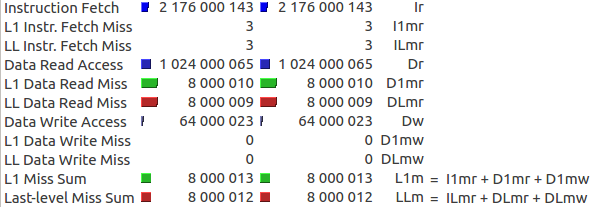
\includegraphics[scale = 0.5]{4_15_1.png} \par
\end{center}
Resultados del cachegrind con una matriz de 8 x 8,000,000 \par
\begin{center}
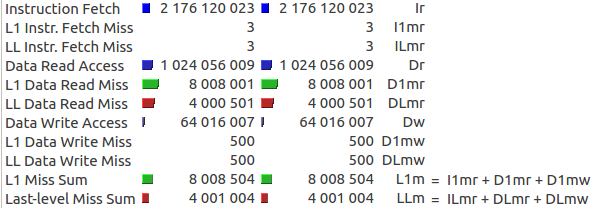
\includegraphics[scale = 0.5]{4_15_2.png} \par
\end{center}
Resultados del cachegrind con una matriz de 8000 x 8000 \par
\begin{center}
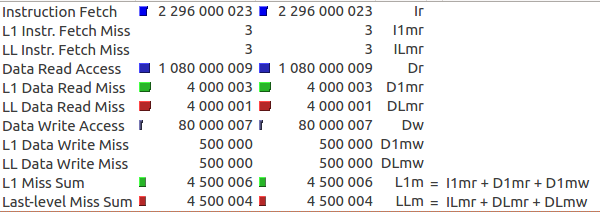
\includegraphics[scale = 0.5]{4_15_3.png} \par
\end{center}
resultados del cachegrind con una matriz de 8,000,000 x 8

\begin{enumerate}
 \item Para el caso uno fueron 0, para el caso dos fueron 500, y para el caso tres fueron 500,000.
 \item Para el caso uno fueron 0, para el caso dos fueron 500, y para el caso tres fueron 500,000.
 \item En el tercer caso es donde ocurren más write-misses. En nuestro caso, con k = 8, el vector resultante
 va a ser de un tamaño de 8,000,000 elementos, y cada uno tiene que ser creado y sobrescrito, por esta razón
 se dan más cache misses en el caso tres.
 \item Para el caso uno fueron 8,000,010, para el caso dos fueron 8,008,001, y para el caso tres fueron 4,000,003.
 \item Para el caso uno fueron 8,000,009, para el caso dos fueron 4,000,501, y para el caso tres fueron 4.000.001.
 \item En el primer caso se dan más read-misses. Porque el tamaño de cada fila de la matrix es 8,000,000, muy grande
 para caber en una línea de cache, por lo tanto, se dan más cache misses en el caso uno. 
 \item La tabla muestra los tiempos obtenidos (En segundos). La entrada más lenta es la matriz de 8,000,000 x 8 y la más rápida
 es la matriz de 8000 x 8000. Haciendo referencia a los resultados obtenidos por el cachegrind, la primera entrada es más lenta
 porque tiene casi el doble de read-misses que las otras entradas, y la segunda entrada es la más rápida porque es la que mejor
 maneja los cache misses.
 
 \begin{center}
\begin{tabular}{|c|c|c|c|}\hline
 & \textbf{8,000,000x8} & \textbf{8000x8000} & \textbf{8x8,000,000}\\\hline
\textbf{Tiempos} & 0.411758 & 0.353235 & 0.375181\\\hline
 \end{tabular}
 \end{center}
 
\end{enumerate}


\item \textbf{Recall the matrix-vector multiplication example with the 8000 x 8000 input. Suppose that the program
is run with four threads, and thread 0 and thread 2 are assigned to different processors. If a cache line contains 64 
bytes or eight double, is it possible for false sharing between threads 0 and 2 to occur for any part of the vector y? Why?
What about if thread 0 and thread 3 are assigned to different processors–is it possible for false sharing to occur between
them for any part of y ?}

En ninguno de los dos casos ocurre un \textit{false sharing}, porque la línea de caché es muy pequeña para que contenga partes
de dos procesos con elementos tan separados. Podría ocurrir un \textit{false sharing} si es que la línea de cache es mucho más grande,
o el tamaño de la matriz es mucho más pequeña, o los hilos tienen valores contiguos.

\item{ \textbf{Recall the matrix-vector multiplication example with an 8 x 8, 000, 000 matrix. Suppose that double use 8 bytes
of memory and that a cache line is 64 bytes. Also suppose that our system consists of two dual-core processors.}

\begin{enumerate}
 \item \textbf{What is the minimum number of cache lines that are needed to store the vector y?}
 \item \textbf{What is the maximum number of cache lines that are needed to store the vector y?}
 \item \textbf{If the boundaries of cache lines always coincide with the boundaries of 8-byte double, in how many different ways can
 the components of y be assigned to cache lines?}
 \item \textbf{If we only consider which pairs of threads share a processor, in how many different ways can four
 threads be assigned to the processors in our computer? Here we’re assuming that cores on the same processor share a
 cache.}
 \item \textbf{Is there an assignment of components to cache lines and threads to processors that will result in no
 falses sharing in our example? In other words, is it possible that the threads assigned to one processor will have their
 components of y in one cache line, and the threads assigned to the other processor will have their components in a different
 cache line?}
 \item \textbf{How many assignments of components to cache lines and threads to processors are there?}
 \item \textbf{Of these assignments, how many will result in no false sharing?}
\end{enumerate}
}

\begin{enumerate}
 \item El tamaño del vector sería de 8. Sólo necesitarías una línea de cache para guardar ese vector.
 \item En el peor de los casos, necesitarías 8 lineas de caché para guardar todo el vector.
 \item 
 \item Podrían distribuirse cada dos, 0 y 1, 2 y 3, 0 y 2, 0 y 3, 1 y 2, 1 y 3.
 \item Ya que todo el vector puede entrar en una línea de cache, es muy difícil no tener \textit{false sharing} cuando
 se están usando los dos procesadores. En este caso, si se quiere evitar el \textit{false sharing}, el programa debería correr
 en un solo procesador.
 \item Hay varias, pero todas utilizan una sola linea de cache para todo el vector.
 \item Todas resultan en un \textit{false sharing}
\end{enumerate}


\item{
\begin{enumerate}
 \item \textbf{Modify the matrix-vector multiplication program so that it pads the vector y when there’s a possibility of
 false sharing. The padding should be done so that if the threads execute in lock-step, there’s no possibility that
 a single cache line containing an element of y will be shared by two or more threads. Suppose, for example, that a cache
 line stores eight double and we run the program with four threads. If we allocate storage for at least 48 double in y, then,
 on each pass through the for i loop, there’s no possibility that two threads will simultaneously access the same cache line.}
 \item \textbf{Modify the matrix-vector multiplication so that each thread uses private storage for its part of y during
 the for i loop. When a thread is done computing its part of y, it should copy its private storage into the shared variable.}
 \item \textbf{How does the performance of these two alternatives compare to the original program? How do they compare to each other?}
\end{enumerate}
}

\begin{center}
\begin{tabular}{|c|c|c|c|c|c|}\hline
\textbf{comm\_sz} & \textbf{1024} & \textbf{2048} & \textbf{4096} & \textbf{8192} & \textbf{16384}\\\hline
\textbf{1} & 0.007907 & 0.025013 & 0.096203 & 0.570424 & 1.944847\\\hline
\textbf{2} & 0.004809 & 0.016058 & 0.090328 & 0.393538 & 1.416607\\\hline
\textbf{4} & 0.004968 & 0.015407 & 0.060883 & 0.31595 & 1.240008\\\hline
\textbf{8} & 0.004961 & 0.015987 & 0.057735 & 0.280157 & 1.110168\\\hline
\textbf{16} & 0.0046 & 0.015397 & 0.056802 & 0.26154 & 1.049518\\\hline
\end{tabular}
\end{center}


\begin{center}
\begin{tabular}{|c|c|c|c|c|c|}\hline
\textbf{comm\_sz} & \textbf{1024} & \textbf{2048} & \textbf{4096} & \textbf{8192} & \textbf{16384}\\\hline
\textbf{1} & 0.014156 & 0.02562 & 0.092135 & 0.507041 & 6.884835\\\hline
\textbf{2} & 0.00675 & 0.022663 & 0.06244 & 0.391432 & 2.087214\\\hline
\textbf{4} & 0.004831 & 0.017741 & 0.058678 & 0.322038 & 1.07533\\\hline
\textbf{8} & 0.004692 & 0.015789 & 0.056342 & 0.286739 & 0.981418\\\hline
\textbf{16} & 0.004327 & 0.015324 & 0.056418 & 0.272768 & 0.940279\\\hline
\end{tabular}
\end{center}



\item \textbf{Although strtok\_r is thread-safe, it has the rather unfortunate property that it gratuitously modifies the
input string. Write a tokenizer that is thread-safe and doesn’t modify the input string.}

\begin{lstlisting}

char * my_strtock(char my_line[], int size, int count){
	int i = 0;
	int c = -1;
	int n = 0;
	for(i = 0; i < size; i++){
		if(my_line[i] == ' ' || my_line[i] == '\n'){
			c++;
			if(c == count) break;
			if(my_line[i] == '\n' && c != count) return NULL;
			n = 0;
		} 
		else n++;
	}
	char * res = malloc(n);
	memcpy(res,&my_line[i - n],n);
	return res;
}
\end{lstlisting}


\end{enumerate}
\end{document}
